In the previous chapters, we only considered uni-variable functions, i.e. functions that takes one number as input.  However, in practice, the quantities we are interested in may be related to serveral variables.  For example, suppose we would like to know our net income $I$ in manufacturing and selling a type of product.  The net income would depend on several variables, including the unit cost for manufacturing the product ($C$), the unit price of the product ($P$), and the quantity of product sold ($Q$).  Therefore, we have 
\[I = (P-C)Q := g(P,C,Q)\]
Here, $g$ would then be a function that takes three numbers as input.  

Previously when we set out to visualize a uni-variable function, say $f(x)$, we would plot $y = f(x)$ on a Cartesian plane using curve sketching techniques.  For functions of several variables, when the number of inputs is greater of equal to $3$, then it is quite challenging to visualize the function.  However, in the special case where the number of inputs is $2$, i.e. a function like $f(x,y)$, we can visualize the function by plotting $z = f(x, y)$ as a three-dimensional surface, where the two inputs $x$, $y$ serve as the $x$- and $y$-coordinates, and the function value $f(x,y)$ serves as the $z$-coordinate.  With the advent of computer graphics, graphing a 3-D plot has been easier than ever (eg. using Wolfram on-line services).  However, in absence of 3-D graphing utilities, we can still figure out how the function approximately looks like using the following techniques

\begin{enumerate}
    \item \underline{Traces on planes parallel to the $yz$- and $xz$-plane}: When the $x$ input in $f(x, y)$ is treated as a fixed constant $x_0$, we have $z = f(x_0, y)$, which now becomes a uni-variable function that can be plotted on a Cartesian plane.  The curve plotted is actually the trace of $f(x, y)$ when sectioned with the plane $x = x_0$, which is a plane perpendicular to the $x$-axis.  For example, in the left panel of the graph below, the section made by $x = x_0$ results in a trace of a parabola.  Similarly, we may treat the $y$ input as a fixed constant $y_0$, which results in a trace of the surface sectioned by $y=y_0$, a plane perpendicular to the $y$-axis. 
    \item \underline{Contour map}: We can also section the surface along planes that are parallel to the $xy$-plane.  That is, for a given value of $z_0$, we find all points $(x,y)$ that satisfied $f(x,y) = z_0$ and graph the trace on the Cartesian plane.  What is great about contour map is that, as long as the function $f(x,y)$ is differentiable everywhere (we will talk about the derivatives for functions of several variables in a bit), we can pick a bunch of possible values of $z$ and graph all their section traces on the $xy$-plane, and these traces would not intersect with each other.  For example, in the right panel of the graph below, the section traces for $z=1, 2, 3, 4$ are graphed on the Cartesian plane, which form a bunch of concentric circle.  Also notice that although we are plotting traces of equal spacing of $z$, the concentric circle are closer and closer to each other as $z$ gets larger.  This implies that the surface is steeper far away from the origin point and gentler near the origin point.  This kind of plot is called the contour map, and is widely used in geographic maps. 
\end{enumerate}

\begin{figure}[ht]
    \centering
    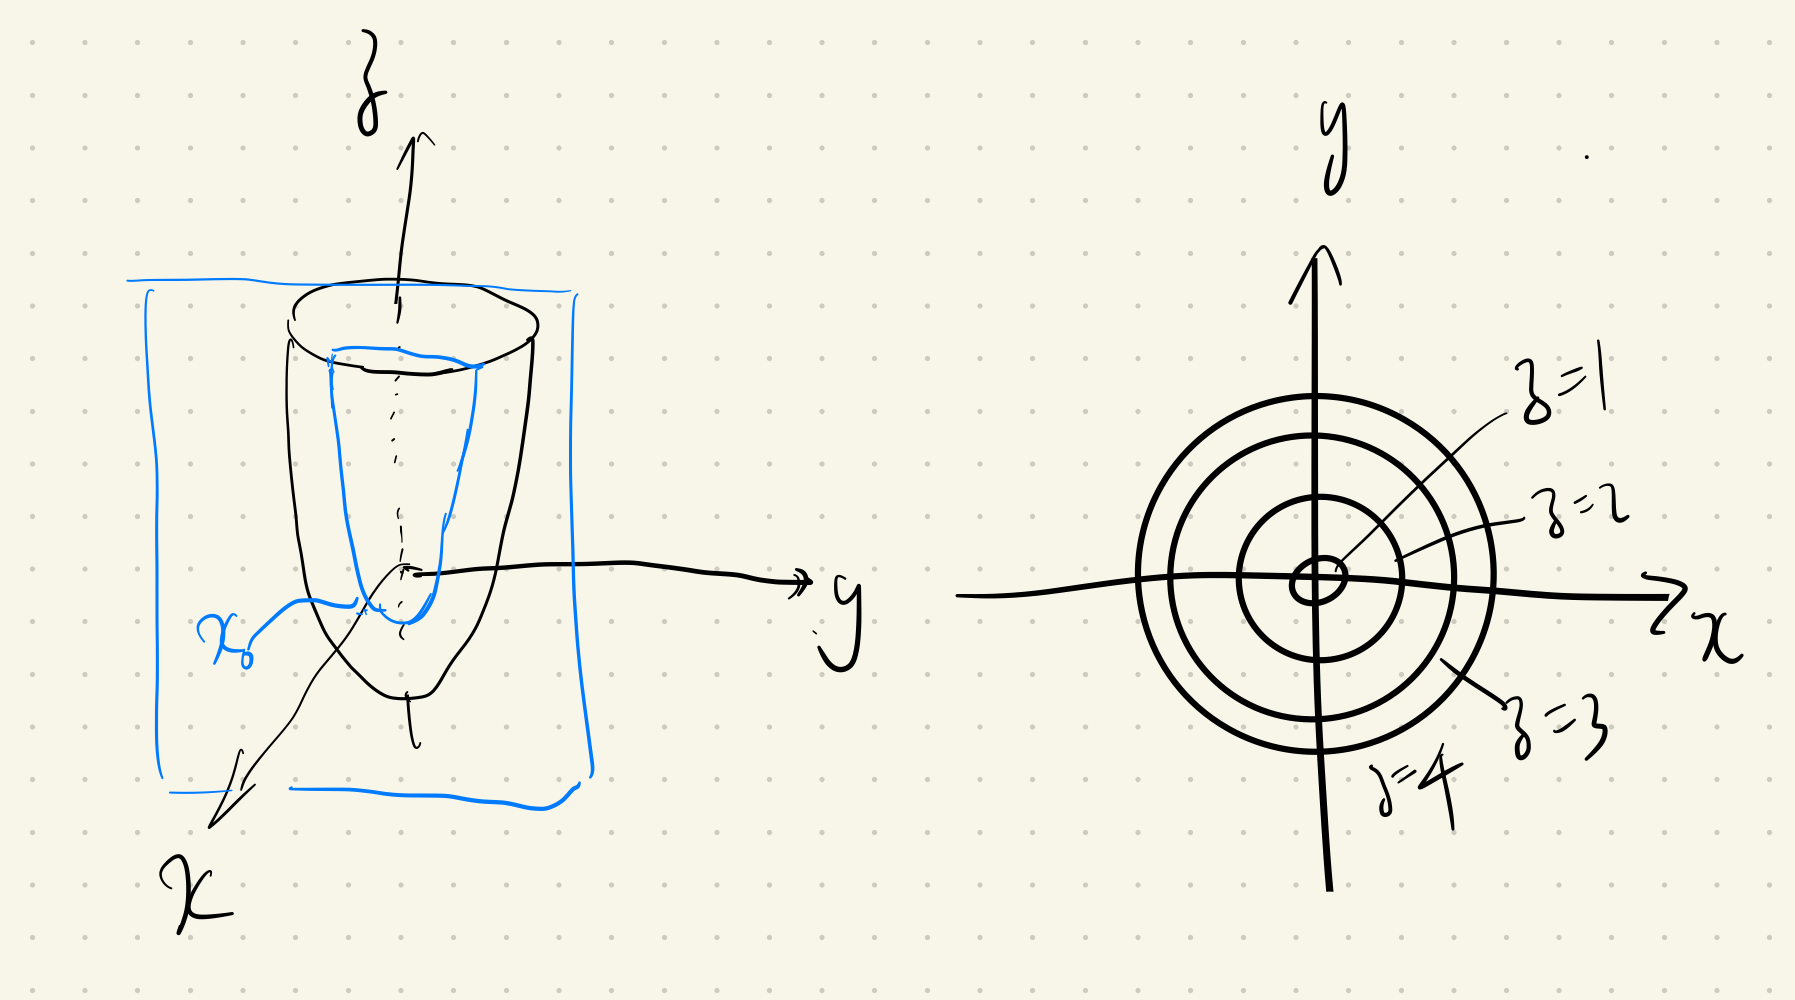
\includegraphics[width = 0.7\textwidth]{figures/chap 08/3D-graph.png}
\end{figure}

\section{Partial derivatives}
When we were dealing with univariable functions, we used derivatives to evaluate the slope of their tangent lines at a certain point, which reflects the rate of change of these functions at that very point.  In functions of two variables, we can still try to evaluate the rate of change of these functions.  What is different from univariable functions is that, for a univariable function, say, $f(x)$, when we are moving a tiny bit away from $(x_0, f(x_0))$, we can only go to $(x_0 + \delta x, f(x_0+ \delta x))$ or $(x_0 - \delta x, f(x_0 - \delta x))$, both of which have the same rate of change relative to $(x_0, f(x_0))$ as long as $f(x)$ is continuous.  However, for a function of two variables, say, $g(x,y)$, for every point on the surface $(x_0, y_0, f(x_0, y_0))$, there are countless direction we can move away from this point, and each direction would have a different rate of change.  

For example, suppose $g(x,y) = x^2 - xy$, and we are trying to find the derivative of $g$ at $(x,y) = (1,2)$.  In the calculation of the derivative, if we are moving away from $(1,2)$ along the direction parallel to $x$-axis, then we are essentially fixing the $y$-coordinate at $2$ while moving the $x$-coordinate.  Therefore, the trace of our movement would be on the plane $y=2$ with $z = g(x,2) = x^2 - 2x$, and the derivative would be 
\[\frac{d}{dx}g(x,0)\Big|_{x=1} = 2x-2|_{x=1} = 0\]
In contrast, if we are moving away from $(1,2)$ along the parallel the $y$-axis, then we are fixing the $x$-coordinate at $1$ while moving the $y$-coordinate.  So the trace of our movement would be on the plane $x=1$ with $z = g(1,y) = 1-y$, and the derivative would be
\[\frac{d}{dy}g(1,y)\Big|_{y=2} = -1|_{y=2} = -1\] 
We can see that moving toward different directions can give us different values of the derivative.  Therefore, before we evaluate the derivative of a function of two variables, we have to specify which direction we are moving away from the point of interest.  Two most obvious directions, as we have demonstrated above, are along the direction parallel to the $x$-axis (holding the $y$-coordinate as constant) and along the direction parallel to the $y$-axis (holding the $x$-coordinate as constant).  These directions lead to the two first-order partial derivatives of the function, defined as below:

\begin{defi}[Partial Derivatives of Functions of Two Variables]{def: partial}
    Let $f(x,y)$ be a continous function, then the first partial derivative of $f$ with respect to $x$ and $y$ are defined as
    \begin{align*}
        \frac{\p f}{\p x} := f_x(x,y) &:= \lim_{h \rightarrow 0} \frac{f(x+h,y)-f(x,y)}{h}\\
        \frac{\p f}{\p y} := f_y(x, y) &:= \lim_{h \rightarrow 0} \frac{f(x,y+h)-f(x,y)}{h}
    \end{align*}
    And the value of the partial derivatives at $(x_0, y_0)$ are denoted as
    \[\frac{\p f}{\p x}\Big|_{(x_0,y_0)} := f_x(x_0, y_0) \qquad\qquad \frac{\p f}{\p y}\Big|_{(x_0,y_0)} := f_y(x_0, y_0)\] 
\end{defi}

Although the definition of partial derivatives seems cumbersome, luckily, the way to derive them is simple: treat the input that is not to be differentiated as constant.  For example, previously we had $g(x, y) = x^2-xy$.  To derive $\p g/\p x$ and its value at $(1,2)$, we can then treat $y$ as a "constant" and differentiate with respect to $y$, which yields
\[\frac{\partial g}{\partial x} = 2x - y \qquad \frac{\partial g}{\partial x}\Big|_{(1,2)} = 2 \cdot 1 - 2 = 0\]
Likewise, we can derive the derivative at $(1,2)$ in the direction parallel to the $y$-axis by
\[\frac{\partial g}{\partial y} = 0 - x = -x \qquad \frac{\partial g}{\partial y}\Big|_{(1,2)} = -1\]
Both values for partial derivatives are exactly what we have derived previously.  We will further demonstrate how first-order partial derivatives are evaluated in the following examples:

\begin{eg}[]{eg: first_partial}
    Suppose a surface in a three-dimensionsal space can be described by $z = f(x,y) = (xy)^x$.
    \begin{enumerate}[a)]
        \item Find the first-order partial derivatives of $f$ with respect to $x$ and $y$.
        \item Evaluate the slope of $f(x,y)$ at $(1,e)$ in the direction parallel to the $x$-axis.
    \end{enumerate}
\end{eg}

\begin{egsol}[]{egsol: first_partial}
    \begin{enumerate}[a)]
        \item For the partial derivative with respect to $x$, we try $y$ as "constant" and yield
        \begin{align*}
            \frac{\p f}{\p x} = \frac{\p}{\p x} (xy)^x&= \frac{\p}{\p x} (e^{\ln(xy)})^x &\\
            &= \frac{\p}{\p x} e^{x \ln(xy)}&\\
            &= e^{x \ln(xy)} \frac{\p}{\p x} (x \ln (xy))&\text{(Chain rule)}\\
            &= (xy)^x \Big[\ln(xy) + x \cdot \frac{1}{x}\Big]&\text{(Product rule)}\\
            &= (xy)^x(\ln(xy)+1)& 
        \end{align*}
        Likewise, for the partial derivative with respect to $y$:
        \[\frac{\p f}{\p y} = \frac{\p}{\p y}(xy)^x = \frac{\p}{\p y} x^x y^x = x^x \cdot x \cdot y^{x-1} = x^{x+1}y^{x-1}\]
        \item The slope of $f(x,y)$ at $(1,e)$ in the direction parallel to the $x$-axis is exactly the definition of $f_x(1,e)$, which can be evaluated by
        \[\frac{\p f}{\p x}\Big|_{(1,e)} = (1 \cdot e)^1 (\ln(1 \cdot e) + 1) = e \cdot (1+1) = 2e\]
    \end{enumerate}
\end{egsol}

\begin{ex}[]{ex: first_partial}
    Let the demand functions for two products $A$ and $B$, denoted as $q_A(p_A, p_B)$ and $q_B(p_A, p_B)$, be functions of the price of A ($p_A$) and price of B ($p_B$).  The two products are said to be \textit{complemetary} when 
    \[\frac{\p q_A}{\p p_B} < 0 \qquad \text{and} \qquad \frac{\p q_B}{\p p_A} < 0\]
    The two products are said to be \textit{substitutes} when 
    \[\frac{\p q_A}{\p p_B} > 0 \qquad \text{and} \qquad \frac{\p q_B}{\p p_A} > 0\]
    Suppose now we have 
    \begin{align*}
        q_A &= 180 - 2.5 p_A + 3 p_B\\
        q_B &= 200 + 1.5 p_A - 0.5 p_B 
    \end{align*}
    Determine if $A$ and $B$ are complementary, substitutes, or neither.
\end{ex}

\begin{exsol}[]{exsol: first_partial}
    Based on the definition of $q_A$ and $q_B$, we have the following partial derivatives:
    \begin{align*}
        \frac{\p q_A}{\p p_B} &= 3\\
        \frac{\p q_B}{\p p_A} &= 1.5
    \end{align*}
    Since both partial derivatives are positive, $A$ and $B$ are \textit{substitutes}. 
\end{exsol}

In Definition \ref{def: partial}, we only defined the partial derivatives for functions of two variables.  This definition can be readily extended to functions of arbitrary number of variables as follows:

\begin{defi}[Partial Derivatives of Functions of Several Variables]{}
    Let $f(x_1, x_2, ..., x_p)$ be a continous function, then the first partial derivative of $f$ with respect to $x_j$ is defined as
    \[\frac{\p f}{\p x_j} := \lim_{h \rightarrow 0} \frac{f(x_1, x_2, ..., x_{j-1}, x_j+h, x_{j+1}, ... ,x_p)-f(x_1, x_2, ..., x_{j-1}, x_j, x_{j+1}, ... ,x_p)}{h}\]
\end{defi}

The recipe for deriving the partial derivative is exactly the same: treat all variables other than $x_j$ as constant and differentiate the function with respect to $x_j$.  For example, suppose we have $f(x,y,z,t) = xyz + yzt^2 + e^{xzt}$, then the partial derivative of $f$ with respect to $x$ is 
\[\frac{\p f}{\p x} = yz + 0 + e^{xzt} \cdot zt = yz + zte^{xzt}\]

Up until now, we have shown how to evaluate the first-order partial derivatives for functions of several variables.  As with ordinary derivatives, it also possible to do partial differentiation repeatedly to a function to obtain its higher-order partial derivatives.  However, note that since we have severval variables available for partial differentiation, we have to specify which variables and in what order do we want to carry out the partial differentiations.  For example, for a function of two variables $f(x,y)$, there are four ways to take its second-order partial derivative, defined with the notations below:

\begin{align*}
    &\frac{\p}{\p x}\Big(\frac{\p f}{\p x}\Big) := \frac{\p^2 f}{\p x^2} := f_{xx} := (f_x)_x \qquad 
    &\frac{\p}{\p y}\Big(\frac{\p f}{\p x}\Big) := \frac{\p^2 f}{\p y \p x} := f_{xy} := (f_x)_y\\
    &\frac{\p}{\p y}\Big(\frac{\p f}{\p y}\Big) := \frac{\p^2 f}{\p y^2} := f_{yy} := (f_y)_y \qquad &\frac{\p}{\p x}\Big(\frac{\p f}{\p y}\Big) := \frac{\p^2 f}{\p x \p y} := f_{yx} := (f_y)_x
    \\
\end{align*}

The two partial derivatives on the right are called \textit{mixed partial derivatives} since they take partial derivatives of different variables.  Notice that the order of $x$ and $y$ in the "fraction style" notation and "subscript style" notation are different: in the "fraction style" you differentiate in a right-to-left fashion, while in the "subscript style" notation you differentiate in a left-to-right fashion.  This may seem a little bit confusing, but fortunately, \textit{it can be shown that as long as the function has continuous second partial derivatives, the order of partial differentiation does not matter}.  To demonstrate this, lets suppose $f(x,y) = x^2y + xy^3$, then we have
\begin{align*}
    \frac{\p^2 f}{\p x^2} &= \frac{\p}{\p x}\Big(\frac{\p f}{\p x}\Big) = \frac{\p}{\p x}\Big(2xy + y^3\Big) = 2y\\
    \frac{\p^2 f}{\p y^2} &= \frac{\p}{\p y}\Big(\frac{\p f}{\p y}\Big) = \frac{\p}{\p y}\Big(x^2 + 3xy^2\Big) = 6xy\\
    \frac{\p^2 f}{\p y \p x} &= \frac{\p}{\p y}\Big(\frac{\p f}{\p x}\Big) = \frac{\p}{\p y}\Big(2xy + y^3\Big) = 2x + 3y^2\\
    \frac{\p^2 f}{\p x \p y} &= \frac{\p}{\p x}\Big(\frac{\p f}{\p y}\Big) = \frac{\p}{\p x}\Big(x^2 + 3xy^2\Big) = 2x + 3y^2
\end{align*}
which verifies that $f_{xy} = f_{yx}$.

\section{Extrema of Functions of Two Variables}

In single variable calculus, we used derivatives extensively to find the local and global extrema of a function.  For a brief recap, to find all the local extrema for a function $f(x)$, we argued that all local extrema should occur at the \textit{critical points} of the function, which is defined as points where its first derivative $f'(x) = 0$ or does not exist.  Therefore, we find all critical points of the function and check them one-by-one to see if they are local minima, local maxima, or neither.  In the case where a critical point is found by $f'(x) = 0$, we can use the \textit{first derivative test} or \textit{second derivative test} to help us do the checking.  In particular, the second derivative test states that a critical point $x = x_0$ attains local minimum if the second derivative $f''(x_0) > 0$, local maximum if $f''(x_0) < 0$, and no information is available from second derivative if $f''(x_0) = 0$.  Lastly, to find global extrema, we may find all local extrema and compare their function values with the function values at the boundary of the function's domain.  In this section, we will see that can can find the extrema of functions of two variables using methods analogus to what we have done in single variable calculus.

For the sake of completeness, we first provide a formal definition of global and local extrema for functions of two variables: 

\smallskip

\begin{defi}[Extrema of functions of two variables]{def: extrema_multi}
    Suppose $(x_0, y_0)$ is in the domain of $f(x,y)$, let $R_0$ be an region for input where $(x_0, y_0) \in R_0$
    \begin{itemize}
        \item $f$ has a \textbf{global (absolute) maximum} at $(x_0, y_0)$ in $R_0$ if $f(x,y) \le f(x_0,y_0), \forall x \in R_0$ 
        \item $f$ has a \textbf{global (absolute) minimum} at $(x_0, y_0)$ in $R_0$ if $f(x,y) \ge f(x_0,y_0), \forall x \in R_0$ 
        \item $f$ has a \textbf{local (relative) maximum} at $(x_0, y_0))$ in $I_0$ if there exists an circular region $R \subset R_0$ where $(x_0, y_0) \in R$ and $f(x,y) \le f(x_0, y_0), \forall x \in R$ 
        \item $f$ has a \textbf{local (relative) minimum} at $(x_0, y_0))$ in $I_0$ if there exists an circular region $R \subset R_0$ where $(x_0, y_0) \in R$ and $f(x,y) \ge f(x_0, y_0), \forall x \in R$ 
    \end{itemize}
\end{defi}

We can see that based on this definition, a local maximum is like a peak of a mountain, and a local minimum is like a valley.  To make sure that a point $(x_0,y_0)$ attains local maximum for a function $f(x,y)$, we must make sure that points neighboring $(x_0, y_0)$ \textit{at all directions} do not attain greater function value than $(x_0, y_0)$.  We now state the equivalent of Fermat's Interior Extremum Theorem for functions of two variables:

\begin{theo}[Interior Extremum Theorem for Functions of Two Variables]{thm: fermat_multi}
    Suppose $f(x, y)$ attains local extremum at $(x_0, y_0) \in R$, where $R$ is an open region.  If the first partial derivatives of $f(x,y)$ exists in $R$, then $f_x(x_0, y_0) = f_y(x_0, y_0) = 0$.
\end{theo}

The intuition of this theorem is that, if you see $f(x, y)$ as a geographic map measuring the height of each point, then as long as the terrain is smooth (existence of first partial derivatives) within a certain area of the map ($R$), then if you are at a valley or a peak, the ground will be relatively flat at where you stand (zero partial derivative).  However, the converse is not true: when the ground is relative flat near you, it is possible that you are neither at a peak nor a valley.  For example, it is possible that you ascend when you walk forwards and backwards, but descend when you walk to the left or right, which is the case for the point marked as X in the following graph.  This kind of point, where the two partial derivatives evaluate to zero but deos not attain local extremum, is called a \textbf{saddle point}.

\begin{center}
    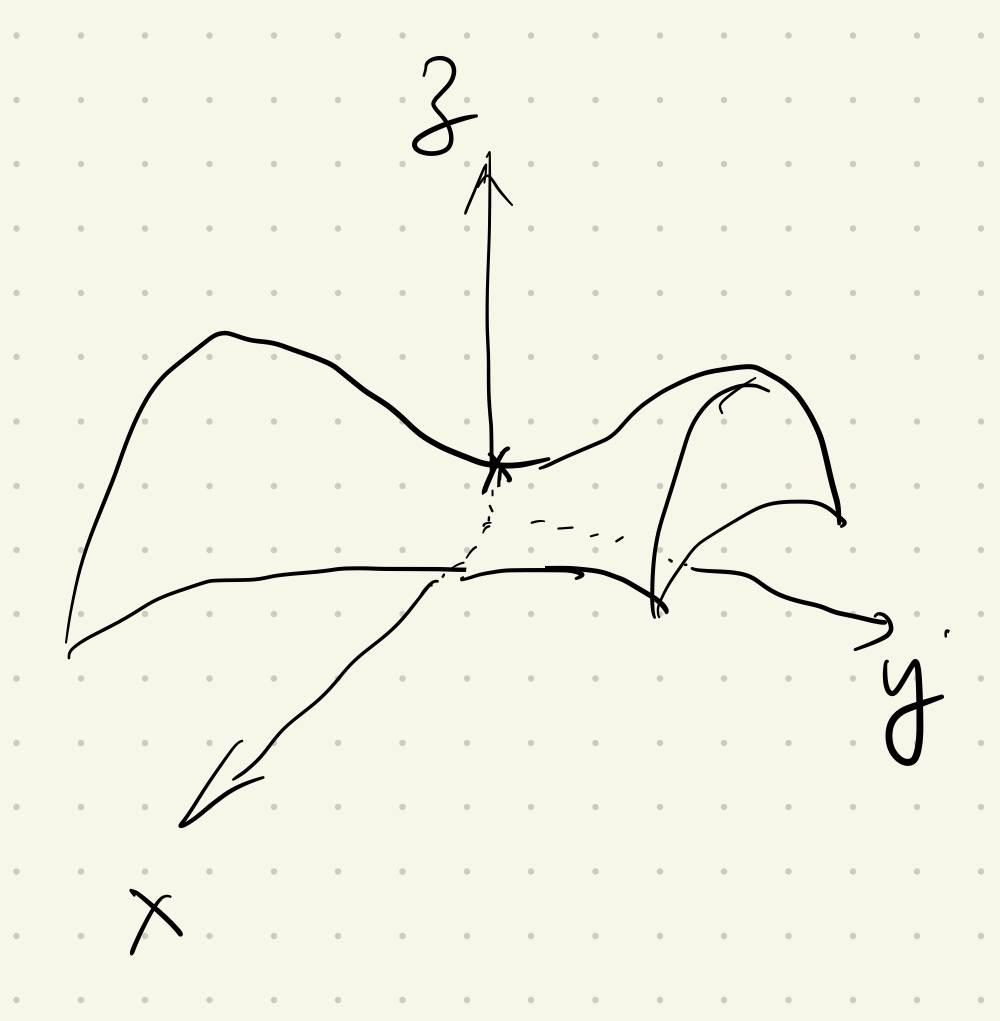
\includegraphics[width = 0.4\textwidth]{figures/chap 08/saddle.png}
\end{center}

Since all local extrema occur at where both partial derivatives evaluates to zero when both partial derivatives exist, we can define critical points of functions of two variables as follows, in order to capture all possible points that can attain local extrema:

\begin{defi}[Critical points of functions of two variables]{def: crit_multi}
    A point $(x_0, y_0)$ in the domain of $f(x, y)$ is termed as a \textit{critical point} for $f(x, y)$ if either of the following holds:
    \begin{enumerate}
        \item $f_x(x_0, y_0) = f_y(x_0, y_0) = 0$
        \item $f_x(x_0, y_0)$ or $f_y(x_0, y_0)$ is undefined at $(x_0, y_0)$
    \end{enumerate}
\end{defi}

After finding the critical points for a function, aside from trying to plot the function around the critical points to assess its behavior at these points, we can use the following second partial derivative test to help us categorize the critical points as long as they are found by letting $f_x(x,y) = f_y(x,y) = 0$.

\begin{theo}[Second Partial Derivative Test for Relative Extrema]{thm: second_partial}
    Suppose a function $f(x, y)$ has continuous second partial derivatives in a region $R$ containing $(x_0, y_0)$ where $f_x(x_0, y_0) = f_y(x_0, y_0) = 0$.  Define the determinant $D$ as
    \[D = f_{xx}(x_0, y_0)f_{yy}(x_0, y_0) - [f_{xy}(x_0, y_0)]^2\]
    \begin{enumerate}
        \item If $D > 0$, then $f$ has a local extrema at $(x_0,y_0)$, and we assess the sign of $f_xx(x_0,y_0)$.
        \begin{enumerate}
            \item If $f_{xx}(x_0,y_0) > 0$, $f$ attains \textbf{local minimum} at $(x_0, y_0)$.
            \item If $f_{xx}(x_0,y_0) < 0$, $f$ attains \textbf{local maxmimum} at $(x_0, y_0)$.
        \end{enumerate}
        \item If $D < 0$, then $(x_0, y_0)$ is a \textbf{saddle point}.
        \item If $D = 0$, the second partial derivatives give no information.
    \end{enumerate}
\end{theo}

Here we will not show how $D$ is derived, but will provide some intuition on why this criterion is needed and why it makes sense.  When $f_{xx}(x_0,y_0)$ and $f_{yy}(x_0,y_0)$ have opposite signs, we can see that $D$ is guaranteed to be less than zero and $(x_0, y_0)$ is a saddle point.  This is reasonable since in the case where $f_{xx}(x_0,y_0) > 0$ and $f_{yy}(x_0,y_0) <0$, the trace of the surface is concave up on $y = y_0$ and concave down on $x = x_0$, which implies that when you are walking from $(x_0, y_0)$, the terrain ascends when you walk parallel to the $x$-axis but decends when you walk parallel to the $y$-axis.  Therefore, it is clear that this point is niether a valley or a peak, so it is a saddle point.  The situtation is similar when $f_{xx}(x_0,y_0) < 0$ and $f_{yy}(x_0,y_0) > 0$.


When both $f_{xx}(x_0,y_0)$ and $f_{yy}(x_0,y_0)$ are positive, the traces of the surface on $x = x_0$ and $y = y_0$ are both concave up, which implies that when you stand at $(x_0, y_0)$ and walk parallel to either the $x$- or $y$-axis, you will find the terrain ascending.  However, this is not sufficient to prove that you are in a valley (i.e. local minimum) since you are still not sure if the terrain would be descending when you walk in a direction not parellel to either the $x$- or $y$-axis.  The additional mixed partial derivative term $[f_{xy}(x_0, y_0)]^2$ can be seen as to provide information on what would happen if you walked diagonally.  When it is large enough to offset the $f_{xx}(x_0,y_0)f_{yy}(x_0,y_0)$ and make $D$ negative, this implies that there are some walking directions where the terrain becomes descending, and the point becomes a saddle point.  Similar arguments can be made in the case where $f_{xx}(x_0,y_0)$ and $f_{yy}(x_0,y_0)$ are both negative.

We will now see how the series of procedures above works in finding local extrema:

\begin{eg}[]{eg: extrema_multi}
    Find the relative extrema and saddle points of $f(x,y) = 6xy - x^6 - y^6$
\end{eg}

\begin{egsol}[]{egsol: extrema_multi}
    We will begin by finding the critical points of $f(x,y)$, with its first-order partial derivatives:
    \begin{align*}
        f_x(x,y) &= 6y - 6x^5\\
        f_y(x,y) &= 6x - 6y^5
    \end{align*}
    Since both partial derivatives are defined under any value of $x$ and $y$, we proceed on find the values of $x$ and $y$ that satisfies $f_x(x,y) = f_y(x,y) = 0$.  This implies 
    \begin{align*}
        y &= x^5\\
        x &= y^5
    \end{align*}
    plugging $x$ with $y^5$ in the first equality yields $y = (y^5)^5 = y^{25}$, so we have $y(y^{24}-1) = 0$, which yields three solutions $y = 0, 1, -1$.  Coupled with the fact that $x=y^5$, we have three critical points: $(0,0)$, $(1,1)$ and $(-1,-1)$.  

    To determine if these critical points are local extrema, saddle points, or neither, we proceed on to the second partial derivative test, which requires us to derive the three second-order partial derivatives:
    \begin{align*}
        f_{xx}(x,y) &= - 30x^4\\
        f_{yy}(x,y) &= - 30y^4\\
        f_{xy}(x,y) &= 6
    \end{align*}
    Therefore, we have the following table, from formula $D = f_{xx}(x,y)f_{yy}(x,y)-[f_{xy}(x,y)]^2$:
    \begin{center}
        \begin{tabular}[ht]{cccccc}
            Critical point & $f_{xx}$ & $f_{yy}$ & $f_{xy}$ & $D$ & Conclusion\\
            \hline
            $(0,0)$ & $0$ & $0$ & $6$ & $-36<0$ & Saddle point\\
            $(1,1)$ & $-30<0$ & $-30$ & $6$ & $864>0$ & Local maximum\\
            $(-1,-1)$ & $-30<0$ & $-30$ & $6$ & $864>0$ & Local maximum
        \end{tabular}
    \end{center}
\end{egsol}

\begin{ex}[]{ex: extrema_multi}
    Suppose there is a rectangular box sitting on the $xy$-plane, with one vertex on the origin point and another on the plane $2x+3y+z = 6$.  Find the maximum volume for the box.
\end{ex}

\begin{exsol}[]{exsol: extrema_multi}
    We can graph the plane using the fact that three points decides a plane: the plane clearly goes through $(3,0,0), (0,2,0)$ and $(0,0,6)$, cutting through the first octant forming a tetrahedron.  Suppose the vertex on the plane is of coordinate $(x,y,z)$, then first since $(x,y,z)$ is on the plane, the three unknowns are not totally free and we have to substitute $z = 6-2x-3y$.  Now since the volume of the box is $V = xyz$, we have
    \[V = xyz = xy(6-2x-3y) = 6xy - 2x^2y-3xy^2\]
    To maximize $V$ with respect to $x$ and $y$, we find the first-order partial derivatives of $V$
    \begin{align*}
        V_x &= 6y - 4xy - 3y^2 = y(6-4x-3y)\\
        V_y &= 6x - 2x^2 - 6xy = x(6-2x-6y)
    \end{align*}
    Since $V_x$ and $V_y$ are always defined, we now try to solve the equation $V_x = V_y = 0$.  From $V_x = 0$, we have $y = 0$ or $6-4x-3y = 0$.  From $V_y = 0$, we have $x = 0$ or $6-2x-6y=0$.  Cross-matching either pair of solutions leads to four solutions for the critical points: $(0, 0), (0, 2), (3, 0), (1, 2/3)$.  

    To determine which these critical points represents a maximum, we proceed on to the second partial derivative test, which requires us to derive the three second-order partial derivatives:
    \begin{align*}
        V_{xx} &= -4y\\
        V_{yy} &= -6x\\
        V_{xy} &= 6-4x-6y
    \end{align*}
    Therefore, we have the following table, from formula $D = V_{xx}V_{yy}-[V_{xy}]^2$:
    \begin{center}
        \begin{tabular}[ht]{cccccc}
            Critical point & $f_{xx}$ & $f_{yy}$ & $f_{xy}$ & $D$ & Conclusion\\
            \hline
            $(0,0)$ & $0$ & $0$ & $6$ & $-36<0$ & Saddle point\\
            $(0,2)$ & $-8$ & $0$ & $-6$ & $-36<0$ & Saddle point\\
            $(3,0)$ & $0$ & $-18$ & $-6$ & $-36<0$ & Saddle point\\
            $(1,2/3)$ & $-8/3 < 0$ & $-6$ & $-2$ & $12>0$ & Local maximum
        \end{tabular}
    \end{center}
    Therefore, the maximum occurs at $(x,y) = (1,2/3)$, and from $z=6-2x-3y$, we get $z = 2$, and the maximum volume is $V = xyz = 1 \cdot 2/3 \cdot 2 = 4/3$.
\end{exsol}

\begin{eg}[]{eg: least_squares_regression}
    Given a set of data of size $n$ observing two variables $(x_1, y_1), (x_2, y_2), ..., (x_n, y_n)$ where $x_i$ are not all identical, the aim of regression is to find a predictor function $f(x)$ so that when we use $f(x_i)$ to predict $y_i$, the \textit{magnitude} of the error $e_i := y_i-f(x_i)$ can be as small as possible.  Since absolute values are more difficult to handle, most commonly we would want to minimize the \textit{square} of the error.  Therefore, least squares regression set out to minimize the following quantity
    \[L = \frac{1}{2}\sum_{i=1}^n e_i^2= \frac{1}{2}\sum_{i=1}^n[y_i - f(x_i)]^2\]
    In the case where $f(x)$ is assume to be a linear function so that $f(x) = \alpha + \beta x$, the quantity to minimize becomes
    \[L(\alpha, \beta) = \frac{1}{2}\sum_{i=1}^n[y_i - (\alpha + \beta x_i)]^2\]
    Show that the following solutions for $\beta$ and $\alpha$ indeed minimizes $L$
    \[\hat{\beta} = \frac{\overline{xy} - \overline{x}~\overline{y}}{\overline{x^2}-\overline{x}^2} \qquad\qquad \hat{\alpha} = \overline{y} - \hat{\beta}\overline{x}\]
    where
    \[\overline{xy} = \frac{1}{n}\sum_{i=1}^n x_i y_i \qquad \overline{x} = \frac{1}{n}\sum_{i=1}^n x_i \qquad \overline{y} = \frac{1}{n}\sum_{i=1}^n y_i  \qquad \overline{x^2} = \frac{1}{n}\sum_{i=1}^n x_i^2\]
\end{eg}

\begin{egsol}[]{egsol: least_squares_regression}
    Note that $L$ is a function of $\alpha$ and $\beta$.  To find the minimizer for $L$, first we try to locate the critical points of $L$.  Expanding the expression within the summation sign, we yield
    \begin{align*}
        &L(\alpha, \beta)\\
        = &\frac{1}{2} \sum_{i=1}^n[y_i - (\alpha + \beta x_i)]^2\\
        = &\frac{1}{2} \sum_{i=1}^n[y_i^2 + \alpha^2 + x_i^2 \beta^2 - 2 y_i \alpha - 2 x_i y_i \beta  +2 x_i \alpha \beta]\\
        = &\Big(\frac{1}{2} \sum_{i=1}^n y_i^2\Big) + \Big(\sum_{i=1}^n 1\Big) \cdot \frac{1}{2} \alpha^2 + \Big(\sum_{i=1}^n x_i^2\Big) \cdot \frac{1}{2}\beta^2 - \Big(\sum_{i=1}^n y_i\Big) \alpha - \Big(\sum_{i=1}^n x_i y_i\Big) \beta + \Big(\sum_{i=1}^n x_i\Big) \alpha \beta\\
        = &\Big(\frac{1}{2} \sum_{i=1}^n y_i^2\Big) + n \cdot \frac{1}{2} \alpha^2 + n \overline{x^2} \cdot \frac{1}{2}\beta^2 - n \overline{y} \alpha - n \overline{xy} \beta + n \overline{x} \alpha \beta
    \end{align*}
    Therefore, the two first-order partial derivatives for $L$ are
    \begin{align*}
        L_\alpha(\alpha, \beta) &= n \alpha - n \overline{y} + n \overline{x} \beta\\
        L_\beta(\alpha, \beta) &= n\overline{x^2} \beta - n \overline{xy} + n \overline{x} \alpha
    \end{align*}
    Since $L_\alpha(\alpha, \beta)$ and $L_\beta(\alpha, \beta)$ are defined for all $\alpha$ and $\beta$, the critical points for $L$ can only occur at where $L_\alpha(\alpha, \beta) = L_\beta(\alpha, \beta) = 0$.  This leads to the following system of equations
    \[\systeme[\alpha\beta]{n\alpha+n\overline{x}\beta=n\overline{y}, n\overline{x}\alpha + n\overline{x^2}\beta = n\overline{xy}}\]
    We divide by $n$ on both sides of the two equations:
    \[\systeme[\alpha\beta]{\alpha+\overline{x}\beta=\overline{y}@\qquad(*), \overline{x}\alpha + \overline{x^2}\beta = \overline{xy}}\]
    And now we can subtract equation (2) by $\overline{x}$ times equation (1) and yield
    \begin{align*}
        (\overline{x^2} - \overline{x}^2)\beta = \overline{xy} - \overline{x} ~ \overline{y}\\
        \beta = \frac{\overline{xy} - \overline{x} ~ \overline{y}}{\overline{x^2} - \overline{x}^2} = \hat{\beta}
    \end{align*}
    Substituting $\beta$ with $\hat{\beta}$ into equation (1), we yield
    \[\alpha = \overline{y} - \overline{x}\hat{\beta} = \hat{\alpha}\]
    Now we know that $(\hat{\alpha}, \hat{\beta})$ is the only critical point for $L$, but we still need to make sure that it attains local minimum, so that $L$ is minmized.  We will thus need to calculate the discriminant $D = L_{\alpha\alpha}(\hat{\alpha}, \hat{\beta})L_{\beta\beta}(\hat{\alpha}, \hat{\beta}) - [L_{\alpha\beta}(\hat{\alpha}, \hat{\beta})]^2$.  Intriguingly, all second partial derivatives for $L$ are actually independent of $\alpha$ and $\beta$:
    \begin{align*}
        L_{\alpha\alpha}(\alpha, \beta) &= n\\
        L_{\beta\beta}(\alpha, \beta) &= n\overline{x^2}\\
        L_{\alpha\beta}(\alpha, \beta) &= n\overline{x}
    \end{align*}
    Therefore, we have
    \begin{align*}
        D &= n \cdot n \overline{x^2} - (n\overline{x})^2\\
        &= n \cdot \sum_{i=1}^n x_i^2 - \Big(\sum_{i=1}^n x_i\Big)^2\\
        &=  \Big(\sum_{i=1}^n 1^2\Big) \cdot \Big(\sum_{i=1}^n x_i^2\Big) - \Big(\sum_{i=1}^n 1 \cdot x_i\Big)^2
    \end{align*}
    The \textit{Cauchy's inequality} states that for any two sets of numbers $a_1, a_2, ..., a_n$ and $b_1, b_2, ..., b_n$, we have the following inequality
    \[\Big(\sum_{i=1}^n a_i^2\Big)\Big(\sum_{i=1}^n b_i^2\Big) \ge \Big(\sum_{i=1}^n a_i b_i\Big)^2\]
    where the equality holds if and only if $a_1/b_1 = a_2/b_2 = ... = a_n/b_n$.  Therefore, here $D \ge 0$ where the equality holds if and only if $x_1 = x_2 = ... = x_n$, which is precluded in the problem.  Consequently, $D > 0$ and $L_{\alpha\alpha} = n > 0$, so the critical point attains local minimum, which implies that it minimizes $L$.
\end{egsol}

\section{Constrained optimization and Lagrange multiplier}
We have seen that for a function of two variables $f(x,y)$, we can find the candidate inputs for local extrema of $f(x,y)$ by first finding its critical points, and assess if $f$ attains local maximum, minimum or neither at each critical point using the discriminant $D$ calculated from second partial derivatives.  However, in some scenarios, we also have an additional constraint on the inputs $(x,y)$.  In this case, the constrained extrema of $f$ may not be identical to its unconstrained extrema.  For example, suppose we have $f(x,y) = x^2+y^2$, then it is trivial that $f$ has a local minimum at $(0,0)$.  But if we add a constraint $xy = 1$, then $(0,0)$ is no longer feasible as an input, and we will have to re-find the local extrema under the constraint.  This kind of problem where we want to find the extrema under one or more constraints is called \textit{constrained optimization}.

One intuitive approach to constrained optimization is to reduce the number of input parameters by substituting one or more parameters with expressions that imply the constraints.  For example, in the example above we have the constraint $xy=1$, so we can substitute $y$ with $1/x$, and the function to optimize becomes a single-variable function
\[f\Big(x, \frac{1}{x}\Big) = x^2 + \frac{1}{x^2}\] 
To optimize this function, we can find its critical points by differentiating it with respect to $x$
\[\frac{d}{dx}f\Big(x, \frac{1}{x}\Big) = 2x - \frac{2}{x^3}\]
The derivative is undefined when $x = 0$ and takes value $0$ when $x = \pm 1$.  The critical point $x=0$ does not work since it is not feasible for the constraint $xy=1$.  The critical point $x=1$, which implies $(x,y) = (1,1)$ under the constraint, obtains local minimum since the second derivative of $f(x, 1/x)$ is positive at $x=1$.  Likewise, the critical point $x = -1$, which implies $(x,y) = (-1,-1)$ under the constraint, also obtains local minimum.  Therefore, we conclude that $f(x,y)$ obtained local minimum at $(x,y) = (1,1)$ and $(-1,-1)$ under the constraint $xy=1$, both taking value $2$.

The approach above breaks down when the constraint is complicated so that is it difficult or impossible to solve for the parameters.  For example, if the constraint is something like $e^(xy) + x^2 + y = 10$, then it is impossible to solve $y$ with expressions of $x$ or solve $x$ with expression of $y$.  In this case, we need a more general strategy to find the constrained extrema.  We first define a function $g(x,y) = xy -1$ so that our constraint is exactly $g(x,y) = 0$.  We then plot $g(x,y) = 0$ and the contour map of $f(x,y)$ on a Cartesian plane as follows:

\begin{figure}[ht]
    \begin{center}
        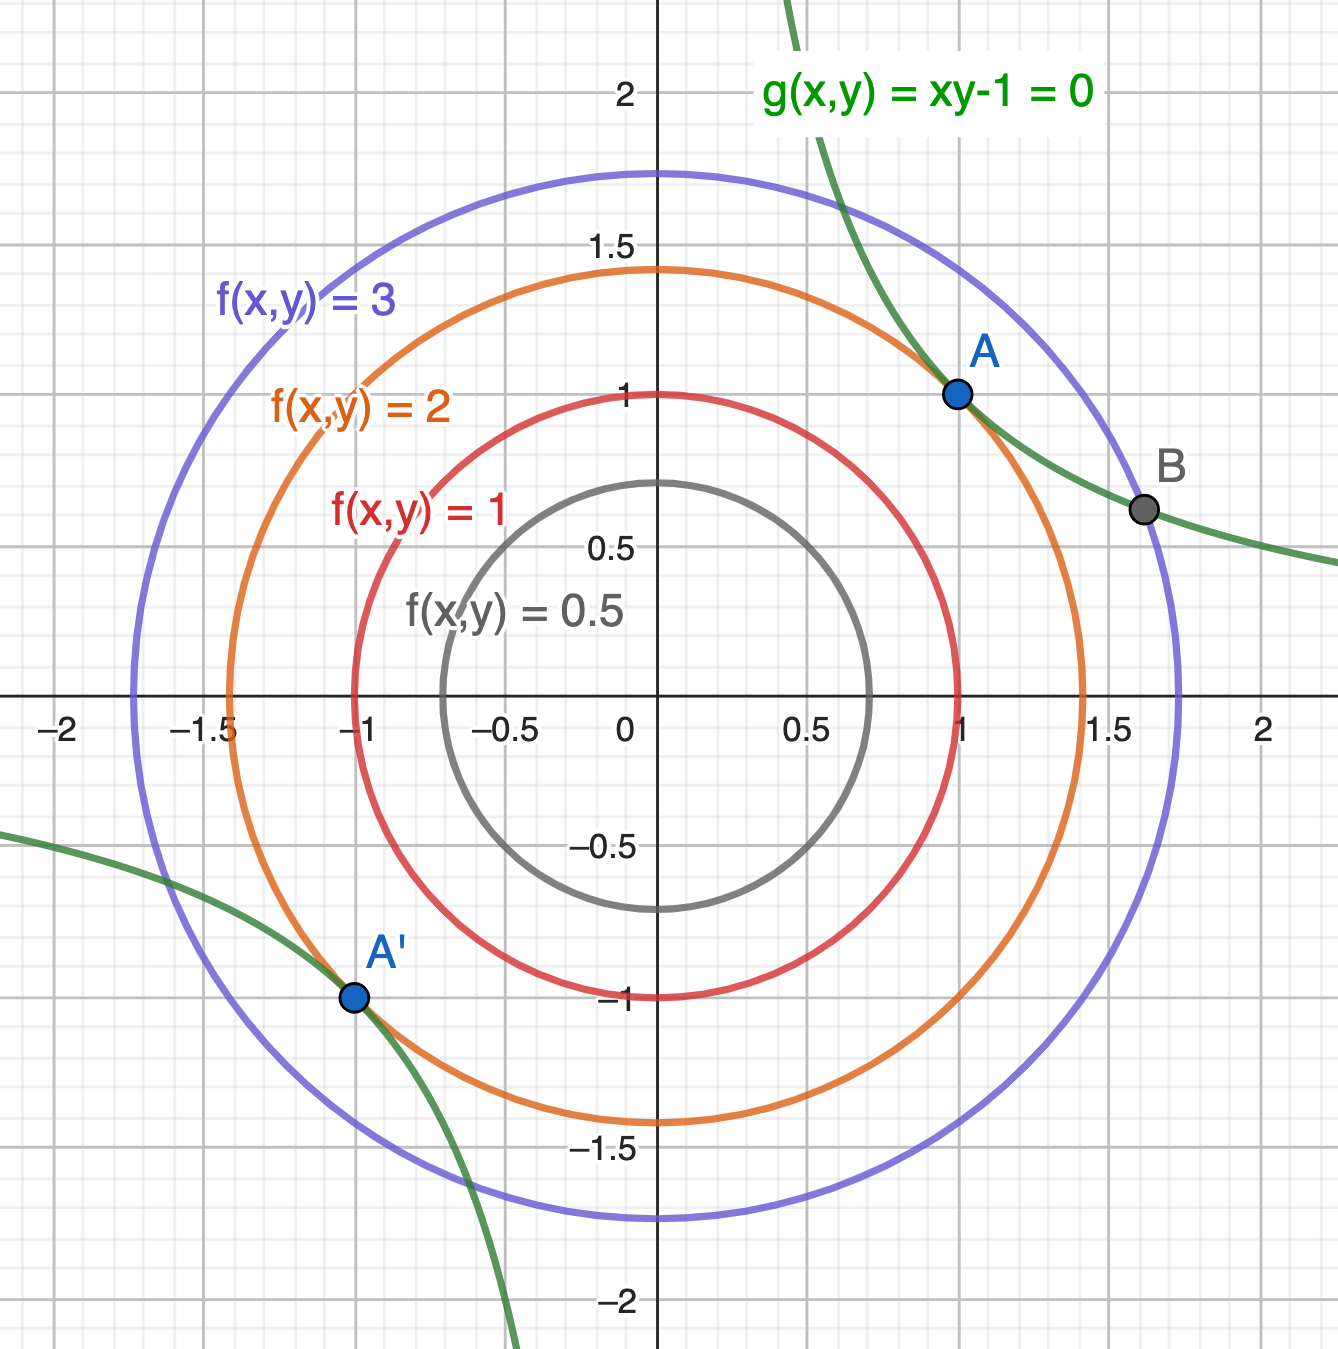
\includegraphics[width = 0.7\textwidth]{figures/chap 08/Lagrange.png}
    \end{center}
\end{figure}

When $f(x,y) < 2$, the contour of $f(x,y)$ does not intersect with $g(x,y) = 0$.  This implies that under the constraint $xy=1$, $f(x,y)$ cannot be smaller than $2$.  When $f(x,y) = 2$, the contour of $f(x,y)$ just kisses $g(x,y) = 0$ at $A(1,1)$ and $A'(-1,-1)$.  Note that this exactly corresponds to our previous results where $f(x,y)$ obtains local minimum of $2$ at $(x,y) = (1,1)$ and $(-1,-1)$.  We will now argue that this is no coincidence.  

Since $g(x,y) = 0$ is our constraint, all feasible inputs lies on its trace.  Therefore, if we start from any feasible input point, say, $B$ on the graph, moving the inputs under the constraints is acually equivalent to sliding it along the curve $g(x,y) = 0$.  Now notice that at point $B$, the contour of $f(x,y)$ is not at the same direction of the curve $g(x,y) = 0$.  This means that even if we are moving away a little bit from $B$ along $g(x,y) = 0$, we are leaving the contour of $f(x,y) = 3$, which implies that $f(x,y)$ is not "flat" near point $B$ along the direction of $g(x,y) = 0$, and thus $f(x,y)$ is not obtaining extremum at point $B$.  

In contrast, at point $A$, the contour of $f(x,y)$ is kissing $g(x,y) = 0$, so they are moving at the same direction at the vicinity of $A$.  That is, if we move away $A$ along $g(x,y)=0$ for a little bit, the value of $f(x,y)$ would not change since its contour is of the same direction, so $A$ is a possible candidate for constrained local extremum.  Notice that this does not guarantee that constrained extremum is obtained at $A$, since it can still be a inflection point or saddle point.  In other words, the contour of $f(x,y)$ and $g(x,y) = 0$ kissing is a necessary condition for a point to be obtaining extremum, but not a sufficient condition.  The rigorous way to determine if the point induces maximum, minimum or neither is more involved and out of scope for this course, but practically you may plug in inputs near the point and argue that it is obtaining maximum when all nearby points results in smaller function values, vice versa.

Now we have argued that the contour of $f(x,y)$ and trace of $g(x,y) = 0$ should go in the same direction locally at the point obtaining extremum.  The pressing question is: how do we come up with a systematic way to find these points?  Now suppose that the point of interest is $(x_0, y_0)$ where $g(x_0, y_0)=0$.  If we move a little bit from $(x_0, y_0)$ to $(x_0 + \Delta x, y_0 + \Delta y)$, what relationship do $\Delta x$ and $\Delta y$ need to satisfy for $(x_0 + \Delta x, y_0 + \Delta y)$ to still stay on $g(x,y) = 0$?  From the definition of partial derivatives, we have
\begin{align*}
    g(x_0 + \Delta x, y_0) &\approx g(x_0,y_0) + g_x(x_0, y_0) \Delta x\\
    g(x_0 + \Delta x, y_0 + \Delta y) &\approx g(x_0 + \Delta x,y_0) + g_y(x_0+\Delta x, y_0) \Delta y\\
    &\approx g(x_0 + \Delta x,y_0) + g_x(x_0, y_0) \Delta y\\
    &\approx g(x_0,y_0) + g_x(x_0, y_0) \Delta x + g_y(x_0, y_0) \Delta y
\end{align*}
Therefore, letting $g(x_0, y_0) = g(x_0 + \Delta x, y_0 + \Delta y) = 0$, we have
\[g_x(x_0, y_0) \Delta x + g_y(x_0, y_0) \Delta y = 0\]
Or, when $g_y(x_0,y_0) \ne 0$,
\[\Delta y = -\frac{g_x(x_0, y_0)}{g_y(x_0, y_0)} \Delta x\]
Now for $f(x,y)$ to obtain extremum at $(x_0, y_0)$, when we move from $(x_0, y_0)$ to $(x_0 + \Delta x, y_0 + \Delta y)$, the value of $f(x,y)$ should remain the same.  Therefore, using arguments similar to above
\begin{align*}
    0 &= g(x_0 + \Delta x, y_0 + \Delta y) - f(x_0,y_0)\\
    &\approx f_x(x_0, y_0) \Delta x + f_y(x_0, y_0) \Delta y\\
    &= f_x(x_0, y_0) \Delta x - f_y(x_0, y_0)\frac{g_x(x_0, y_0)}{g_y(x_0, y_0)} \Delta x\\
    &= \Big[f_x(x_0, y_0) - f_y(x_0, y_0)\frac{g_x(x_0, y_0)}{g_y(x_0, y_0)}\Big] \Delta x
\end{align*}
Since $\Delta x \ne 0$, we have
\[f_x(x_0,y_0) = f_y(x_0, y_0)\frac{g_x(x_0, y_0)}{g_y(x_0, y_0)}\]
\[\frac{f_x(x_0,y_0)}{g_x(x_0,y_0)} = \frac{f_y(x_0, y_0)}{g_y(x_0, y_0)} := \lambda\]
where we denote the ratio as $\lambda$.  We then rearrange the equations and add in the constraint:
\begin{align*}
    f_x(x_0,y_0) - \lambda g_x(x_0,y_0) &= 0\\
    f_y(x_0,y_0) - \lambda g_y(x_0,y_0) &= 0\\
    g(x_0, y_0) &= 0
\end{align*}
Notice that these three equations can be made concise if we define the \textbf{Lagrangian function} as
\[\mathcal{L}(x,y,\lambda) = f(x,y) - \lambda g(x,y)\]
and the three equations become
\begin{align*}
    \mathcal{L}_x(x_0,y_0,\lambda) &= 0\\
    \mathcal{L}_y(x_0,y_0,\lambda) &= 0\\
    \mathcal{L}_\lambda(x_0,y_0,\lambda) &= 0
\end{align*}
This is call the method of \textbf{Lagrange multiplier}, which is extensively used in constrained optimziation.  It can be readily extended to optimization problems for functions of more than two inputs and multiple constraints: Suppose we want to find the local extrema of $f(x_1, x_2, ..., x_p)$ with $k$ constraints, $g_i(x_1, x_2, ..., x_p) = 0$, where $i$ ranges from $1$ to $k$, then we define the Larangian function as follows
\[\mathcal{L}(x_1, x_2, ..., x_p, \lambda_1, \lambda_2, ..., \lambda_k) = f(x_1, x_2, ..., x_p) - \sum_{i=1}^k \lambda_i g_i(x_1, x_2, ..., x_p)\]
Then the candidates for points that obtain extremum can be found by solving
\begin{align*}
    \mathcal{L}_{x_1}(x_1, x_2, ..., x_p, \lambda_1, \lambda_2, ..., \lambda_k) &= 0\\
    \mathcal{L}_{x_2}(x_1, x_2, ..., x_p, \lambda_1, \lambda_2, ..., \lambda_k) &= 0\\
    &\vdots\\
    \mathcal{L}_{x_p}(x_1, x_2, ..., x_p, \lambda_1, \lambda_2, ..., \lambda_k) &= 0\\
    \mathcal{L}_{\lambda_1}(x_1, x_2, ..., x_p, \lambda_1, \lambda_2, ..., \lambda_k) &= 0\\
    \mathcal{L}_{\lambda_2}(x_1, x_2, ..., x_p, \lambda_1, \lambda_2, ..., \lambda_k) &= 0\\
    &\vdots\\
    \mathcal{L}_{\lambda_k}(x_1, x_2, ..., x_p, \lambda_1, \lambda_2, ..., \lambda_k) &= 0
\end{align*}

We will now see how Lagrange multiplier works in our previous example.

\begin{eg}[]{eg: lagrange}
   Find the local extrema of $f(x,y) = x^2 + y^2$ under the constraint $xy = 1$.
\end{eg}

\begin{egsol}[]{egsol: lagrange}
    Using the method of Lagrange multiplier, we first define the constraint function $g(x,y) = xy - 1$ so that the contraint is $g(x,y) = 0$.  Then, we can define the Lagrangian function as 
    \[\mathcal{L}(x,y,\lambda) = f(x,y) - \lambda g(x,y) = x^2 + y^2 - \lambda(xy-1)\]
    Then, the candidate points for local extrema can be found by solving
    \begin{align}
        \mathcal{L}_x(x,y,\lambda) &= 2x - \lambda y = 0 \label{eq: lagrange_x}\\
        \mathcal{L}_y(x,y,\lambda) &= 2y - \lambda x = 0 \label{eq: lagrange_y}\\
        \mathcal{L}_\lambda(x,y,\lambda) &= xy-1 = 0 \label{eq: lagrange_l}
    \end{align}
    From \Cref{eq: lagrange_x}, we have $x = \frac{\lambda}{2}y$, so the $x$ in \Cref{eq: lagrange_y} can be substituted and we yield $2y - \frac{\lambda^2}{2}y = 0$, i.e. $(2+\lambda)(2-\lambda)y = 0$.  Therefore, we have three scenarios:
    \begin{enumerate}
        \item $\lambda = -2$: In this case, both \Cref{eq: lagrange_x,eq: lagrange_y} imply $x = -y$.  So from \Cref{eq: lagrange_l}, $-y^2-1=0$, which has no real solutions, and this root is discarded.
        \item $\lambda = 2$: In this case, both \Cref{eq: lagrange_x,eq: lagrange_y} imply $x = y$.  So from \Cref{eq: lagrange_l}, $y^2-1=0$, which implies $y = 1$ or $-1$.  Given that $x = y$,  $(x,y) = (1,1)$ or $(-1,-1)$.
        \item $y=0$: When $y=0$, \Cref{eq: lagrange_l} can never be fullfilled, so this root is also discarded.
    \end{enumerate}
    Pluggin in $(1,1)$ and $(-1,-1)$ into $f$ and we both yield $2$.  When we plug in points near these points that satisfies the constraint, eg. $(0.9, 1/0.9)$, $(1.1, 1/1.1)$, $(-0.9, -1/0.9)$, $(-1.1, -1/1.1)$, we get values larger than $2$, so we can postulate that $f$ obtains local minimium at these inputs.
 \end{egsol}